\chapter{Introducción y objetivos}
\label{cap:introduccion}

En la actualidad, la empresa BQ se ha especializado en fabricar y distribuir impresoras 3D junto con sus consumibles. En 2013, se creó un departamento de Innovación y Desarrollo, encabezado por Juan González y Alberto Valero. En ese comienzo se distribuye material relacionado con las impresoras 3D para que cualquier persona pueda construirse una impresora 3D. En esta primera etapa, este material no es fabricado por BQ directamente, tan solo realiza la tarea de distribuidor.\\

A medida que BQ adquiere experiencia en el mercado, empieza a crear una línea de investigación para desarrollar sus propias impresoras 3D, como es el caso de la impresora Witbox y la impresora Prusa Hephestos (ver Figura \ref{fig:impresoras_bq}). En este caso BQ tiene un papel importante a lo largo del desarrollo del producto, desde la elección de las características finales del mismo, así como el aspecto final del packaging, es decir, BQ pasa de tener un papel de distribuidor a ser la parte principal del desarrollo del producto.

\begin{figure}[!h]
    \centering
    \begin{subfigure}[b]{0.4\textwidth}
        \centering
        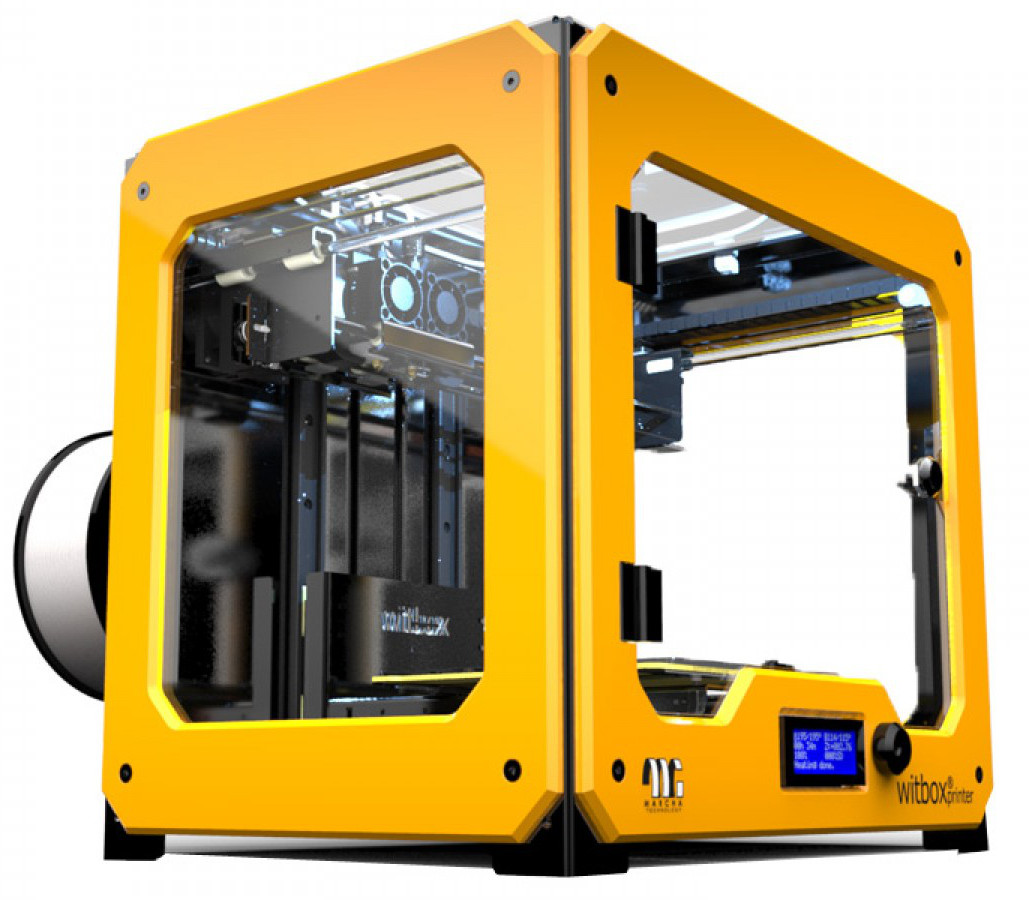
\includegraphics[width=\linewidth]{images/Witbox.jpg}
        \label{fig:estado_witbox}
    \end{subfigure}
    ~
    \begin{subfigure}[b]{0.3\textwidth}
        \centering
        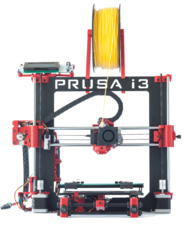
\includegraphics[width=\linewidth]{images/190px-HEPHESTOS.png}
        \label{fig:estado_hephestos}
    \end{subfigure}
    \caption[Impresoras fabricadas por BQ.]{Impresoras fabricadas por BQ. Podemos ver las dos impresoras que desarrolla BQ, a la izquierda, Witbox impresora que ya se vende montada. A la derecha, Prusa Hephestos, se vende en formato kit para que el usuario final la monte (DIY). Fuente \cite{bq}.}
    \label{fig:impresoras_bq}
\end{figure}

A la vez que se venden las impresoras 3D, BQ también vende el principal consumible para que las impresoras 3D puedan funcionar, plástico en forma de filamento. Este plástico se distribuye en unas bobinas (ver Figura \ref{fig:estado_filamento}), en las que está almacenado un hilo continuo de plástico con un diámetro específico, en este caso, $1.75mm$. Al igual que en el caso de las impresoras en un primer momento BQ distribuye filamento fabricado por terceros, pero una vez que BQ tiene un puesto en el mercado de las impresoras 3D, decide entonces crear su propio filamento y tener más controlado la calidad del filamento que vende.

\begin{figure}[!ht]
    \centering
    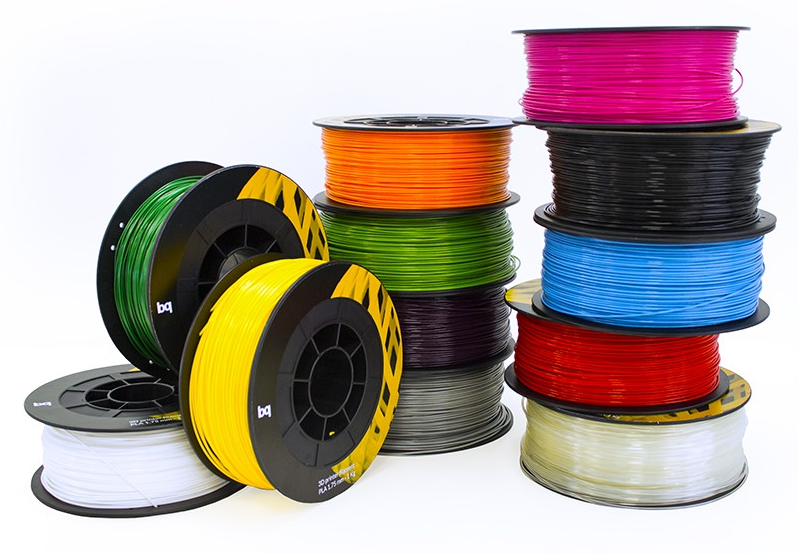
\includegraphics[width=0.5\textwidth]{images/filamento_bq.png}
    \caption[Distintos filamentos de BQ.]{Distintos filamentos de BQ. Fuente \cite{bq}.}
    \label{fig:estado_filamento}
\end{figure}

Por diversos motivos BQ decide sub-contratar el proceso de fabricación a una empresa experta en la extrusión de plásticos pero formando parte en el proceso de calidad del filamento producido. Esta empresa es PESL especialista en extrusión de perfilería de plástico. BQ junto a PESL empiezan a trabajar en la fabricación de un filamento que cumpla las condiciones de calidad necesarias para el proceso de impresión 3D. En una primera aproximación estas condiciones son, el tipo de material y que el diámetro final esté comprendido en un margen de tolerancias.\\

Durante las pruebas iniciales previas a la comercialización del filamento, se aprecia que no todas las bobinas del mismo lote de fabricación tienen la misma calidad, llegando a darse el caso que en una misma bobina, no todo el filamento es igual. El principal problema se encuentra en el diámetro del filamento no es constante (ver Figura \ref{fig:muestra_filamento}).

\begin{figure}[!ht]
    \centering
    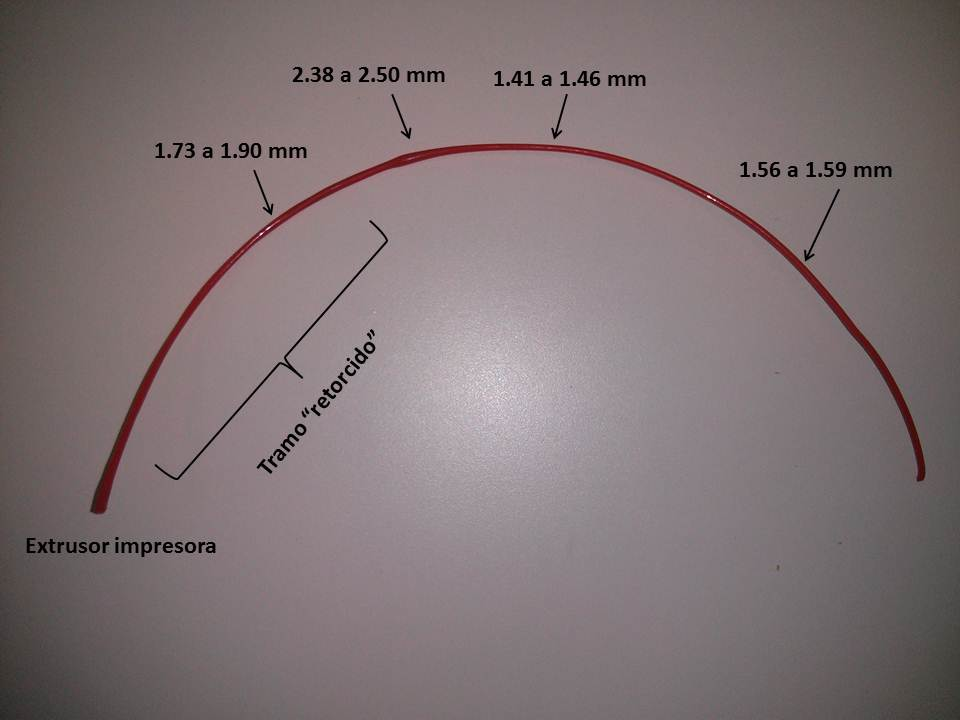
\includegraphics[width=0.6\textwidth]{images/atasco_rojo.jpg}
    \caption[Muestra de filamento con problemas en el diámetro]{Muestra de filamento con problemas en el diámetro. Podemos observar cómo en un tramo de filamento, el diámetro no es constante.}
    \label{fig:muestra_filamento}
\end{figure}

Este problema es importante ya que las impresoras dejan de imprimir pasado un tiempo, puesto que si el diámetro nominal del filamento sobrepasa un determinado rango de valores, tanto por exceso como por déficit, se producen atascos en la impresora. Estos atascos, en el mejor de los casos, sólo supone la limpieza del extrusor de la impresora y se puede volver a utilizar, pero en ocasiones el atasco puede deja inservible el extrusor y es necesario reemplazarlo.\\

Desde BQ se propone instalar un sistema de adquisición de datos que centralice todos los parámetros de producción de filamento como son temperaturas, velocidades de producción y diámetro final del filamento y así tener un sistema de gestión de calidad robusto y escalable en caso de que las líneas de producción aumentasen en un futuro. Sin embargo tras una valoración económica inicial en la que no ser termina de ver claro la aceptación del producto por parte de PESL, se decide afrontar una implementación parcial del sistema de adquisición de datos añadiendo un registro de los diámetros de la producción en un ordenador local e incorporando un elemento mecánico por el cual pasa el filamento. De manera que si este supera un diámetro máximo se parte y la producción se detiene. Adicionalmente el operador puede introducir de forma manual los parámetros de producción menos relevantes del proceso para tener los registros almacenados.\\

Gracias a que cada bobina contiene un código QR en el que, entre otra información, se incluye el número de lote de fabricación, se puede trazar el proceso de fabricación para estudiar los datos obtenidos en caso de ser necesario. Sin embargo al ser una implementación local y poco flexible, el proceso de recuperación de la información para los diversos análisis se dificulta.\\

Cómo finalmente la aceptación del filamento por parte del mercado ha sido buena, se empiezan a aumentar las líneas de extrusión, desde BQ se decide apostar en el desarrollo del sistema de adquisición de datos. Siendo sus requisitos principales:

\begin{itemize}
    \item{Registro de la fecha de fabricación.}
    \item{Registro de las medidas del diámetro final del filamento.}
    \item{Registro de todos los parámetros de fabricación: temperaturas y velocidades}
\end{itemize}

Esta información será almacenada en una base de datos, la cual se podrá acceder de manera remota. Además en caso de que se añadan líneas de extrusión a la fábrica, el sistema será totalmente válido para expandirlo de manera rápida y efectiva.\\

Este trabajo incluye la información necesario para conseguir un primer desarrollo de un sistema de adquisición de datos y demostrar la solución del problema que tenemos. Pasa por diferentes etapas en las que se encuentra buscar qué dispositivo es el más adecuado para llevar el control y, que este, sea estable, robusto y lo más versátil posible, para poder implementarlo en cualquier línea de extrusión. Una vez conseguida la unidad central de control, el siguiente paso será realizar la programación para que el sistema, de forma automática, adquiera los datos que se le indiquen y guarde la información en un medio físico para su posterior análisis.\\

A continuación, se detallan los objetivos a conseguir en el proyecto:

\begin{itemize}
    \item Implementar un sistema capaz de adquirir los parámetros del proceso de fabricación del filamento.
    \item Que el sistema de adquisición pueda ser fácilmente adaptado a cualquier línea de extrusión y sea escalable a cualquier número de línea de extrusión.
    \item Estudio de los datos adquiridos y desarrollo del modelo teórico de la planta.
\end{itemize}
\label{Listado_objetivos}

Una vez que el sistema diseñado sea capaz de almacenar la información, será necesario instalarlo en una línea de extrusión con el fin de servir como herramienta de control de calidad y a su vez que permita la adquisición de datos para poder inferir un modelo de planta, con el que poder empezar a trabajar en reguladores que ayuden a minimizar los errores producidos durante la fabricación de filamento en lazo abierto.\\
\newpage
\section{Organización de este documento}
\label{sec:organizacion}

En el Capítulo 2 desarrollamos conocimientos previos relacionados con el mundo de la impresión 3D, cómo a pesar de ser una tecnología asentada en la industria ha sido en los últimos años cuando se ha difundido en la sociedad.\\

En el Capítulo 3 se analizan las soluciones que otras empresas proponen para el mismo problema y cómo nuestro sistema puede mejorar los distintos sistemas disponibles en el mercado.\\

El Capítulo 4, Desarrollo de la solución propuesta, muestra el trabajo realizado para cumplir el objetivo principal: Planificar las distintas tareas necesarias para el desarrollo del sistema, detallar las herramientas utilizadas y por qué se han decidido usar; y se verá la instalación del sistema en una línea de extrusión de pequeñas dimensiones, para poder comprobar como de válido es nuestro sistema\\

El Capítulo 5 muestra los ensayos realizados para dar validez a que el sistema desarrollado es válido para minimizar el error presentado en la introducción del proyecto.\\

Por último, concluiremos de si el sistema desarrollado cumple el objetivo principal marcado. También veremos los aportaciones que se han derivado a la hora de realizar el proyecto, en forma de pequeños sistemas capaces de solucionar otros problemas que en un primer lugar no eran ámbito de este trabajo final de grado.